\begin{figure}[t]
    \centering
    \begin{tabular}{m{40mm} m{40mm} m{10mm}}
        \begin{minipage}[b]{\linewidth}
            \centering
            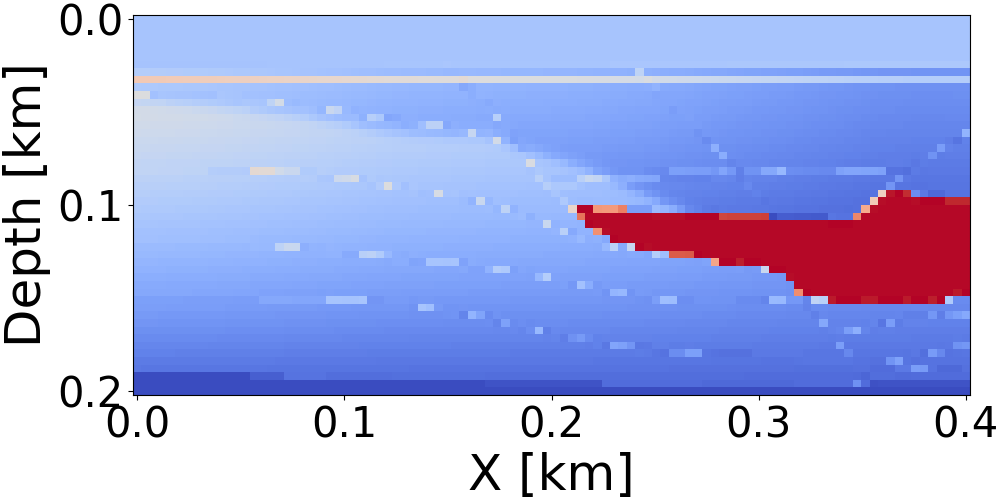
\includegraphics[width=\linewidth]{public/true}
%            \vspace{-9mm}
            \caption*{\raisebox{-3mm}{Ground truth}}
%            \vspace{1mm}
        \end{minipage} &
        \hspace{-5mm}
        \begin{minipage}[b]{\linewidth}
            \centering
            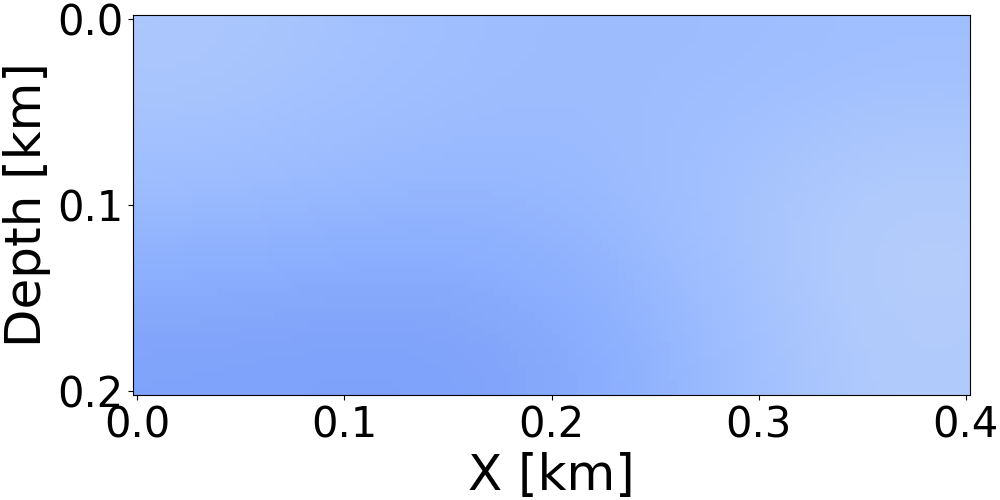
\includegraphics[width=\linewidth]{public/initial}
%            \vspace{-9mm}
            \caption*{\raisebox{-3mm}{Initial model}}
%            \vspace{1mm}
        \end{minipage} &
        \hspace{-8mm}
        \raisebox{3.5mm}{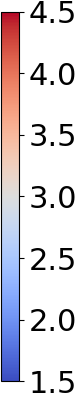
\includegraphics[height=25mm]{public/color-bar}}
    \end{tabular}
%    \vspace{-4mm}
    \caption{The velocity models for experiments.}
%    \vspace{-5mm}
    \vspace{2mm}
    \label{fig:experiment-data}
\end{figure}
